\chapter{Models}
\label{chap:models}
This section exposes the reader to the different model architectures used during the project. We decided not to go for a complex deep learning algorithm such as ResNet\cite{resNet_he2015deep} for simplicity but it would be interesting to try them with more data to see the impact.

\section{Standard 3D CNN}
\label{sec:standard_cnn}

The model we choose for classification is composed of 12 convolutional layers each of size 3 by 3 by 3. The number of output channels gradually increases from 1 (grey-scale) to 32. As we are dealing with 3D images, it is not scalable to increase the number of channels without reducing the image size as it would require a lot of GPU memory. Therefore, we added a MaxPooling layer after every two convolutional layers. This technique is used to reduce the image size, but this is not the only way of reducing the image size. In fact, when performing standard convolution with a kernel of size k.

The output shape in each dimension will be of $s_{out} = \frac{s_{in} - k + 2* pad}{stride} + 1$, where $k$ is the kernel size, $pad$ the added padding and $s_{in}$ the input size. In this work, we focused on building a model that could explain its prediction as much as possible. During the project, we have realized that it was important to keep the shape of the image unchanged after each convolution layer, otherwise, we got some alignment issue between the image and the saliency map once interpolated to the image dimensions. The image is therefore padded with zeros all around in order to prevent it from these artifacts.

Between every layer, we choose to activate the layer output with the classical Relu\cite{relu_10.5555/3104322.3104425} function. The main reason behind this choice is the need for easy interpretability with the FullGrad algorithm (the current implementation only supports the Relu activation function).  
The convolutional layers are good for extracting relevant features for the task. These features are then fed into a classifier composed of two linear layers. A dropout\cite{dropout_10.5555/2627435.2670313} layer has been added in between these layers in order to reduce overfitting. The architecture is summarized in figure~\ref{fig:standard_cnn_model}.

\begin{figure}
    \centering
    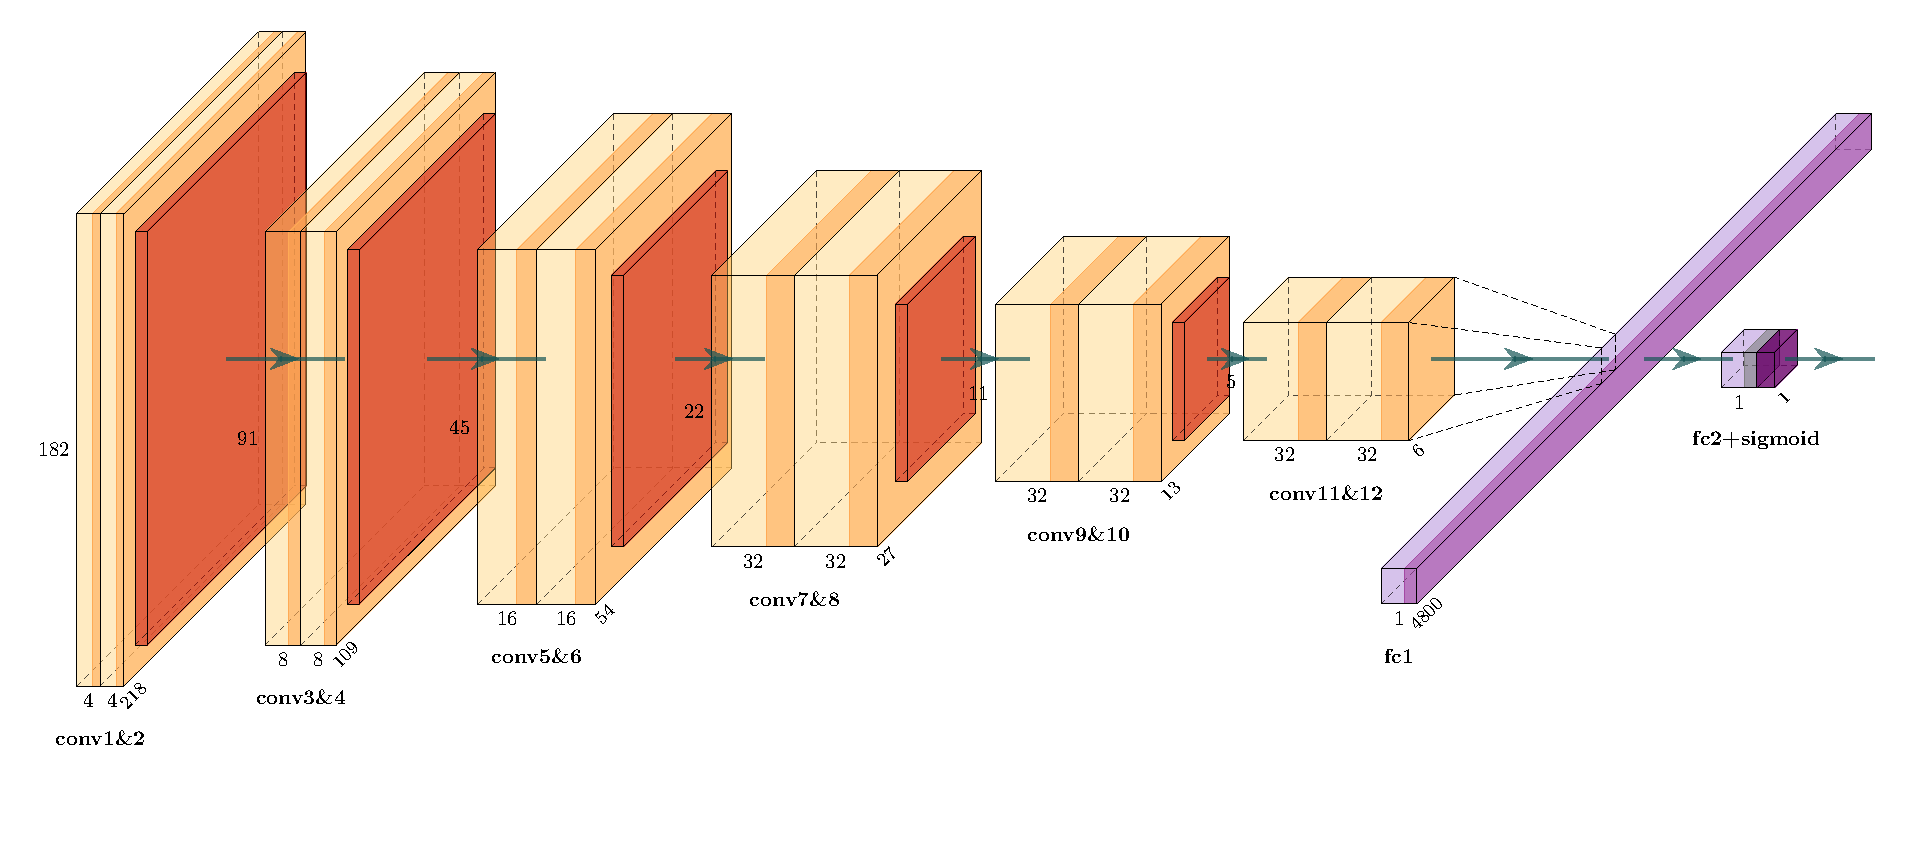
\includegraphics[width=1\linewidth]{figures/models/standard_cnn_model.pdf}
    \caption{Architecture of the implemented network. For visual purpose the MRI image of shape (182, 218, 182) is represented as an image of shape (182, 218).}
    \label{fig:standard_cnn_model}
\end{figure}

\section{3D CNN With Global Average Pooling}

The model described above has quite a lot of parameters to learn especially due to the last linear layers. In fact, when flattening the reduced image it becomes a high-dimmensinal vector. This has the disadvantages of being harder to train and demands a larger amount of training data. As already stated at the time of writing we do not have a lot of data to train our model. 

To overcome this, we slightly changed the design of our network and replaced the flattening layer by a \textit{Global Average Pooling Layer}\cite{GAP_lin2013network} (GAP). This change dramatically reduced the number of parameters of the classifier which allowed us to increase the number of output channels of our features extractor to 128.  

This technique is often performed in computer vision and has the advantage of allowing the network to infer on data of almost any size. By construction, it gives the network a translation invariance property in the opposite of being only equivariant to translation for standard 3D CNN.

With regards to our preprocessing this might, in fact, be a feature not well suited, as all the brain scans are registered into the same space meaning that a specific voxel is going to encode a specific location inside the brain. This global average pooling has, in fact, the disadvantage of losing some spatial location property.


\section{Unbiased Model}
\label{sec:unbias_model}

Often the data has some underlying bias. For example, in the case of Alzheimer’s disease, it appears that old people are more likely to be diagnosed with the disease than young ones (see figure~\ref{fig:OASIS_age_dist}). Experiments on age prediction in annex~\ref{chap:age_pred}, show that age is a hidden feature well present in MRI scan.

\begin{wrapfigure}{r}{0.6\textwidth}
 \centering
 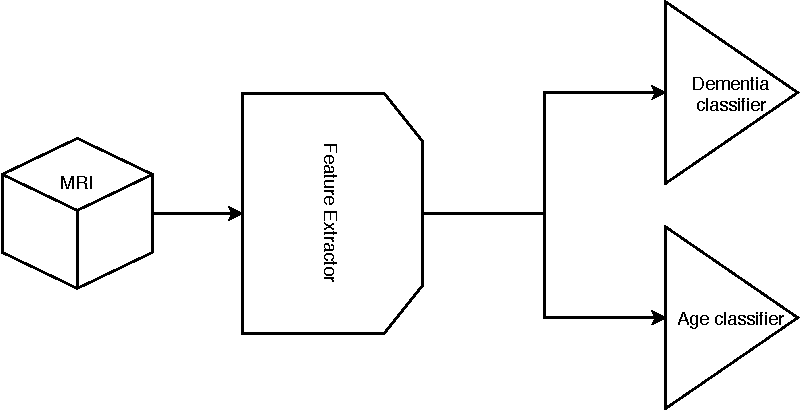
\includegraphics[width=.9\linewidth]{figures/models/Unbias_model.pdf}
 \captionsetup{width=.9\linewidth}
 \caption[UnbiasModelSchema]{Unbiased Model Schema.}
 \label{fig:unbias_model_schema}
\end{wrapfigure}

Such bias can, of course, fool the model, that might be overconfident on classifying old people as having dementia or even worse, young people as healthy just because in the training set demented samples were mostly old people.
Note that by building the model below we are indeed only interested in mitigating the bias due to age, but this model can be easily modified in order to mitigate other potential biases as long as the label is provided for the bias. Examples of other bias might be sex, left- or right-handed, or even the hospital/machine used for scanning.


As illustrated by figure~\ref{fig:unbias_model_schema}, the model is composed of 3 elements. The \textit{feature extractor} extract a fixed number of features from the MRI using convolutional layers in a similar manner as the other models described in chapter~\ref{chap:models}. The \textit{dementia classifier} and \textit{age predictor} are both composed of fully connected layer, with one feature as output. The dementia classifier has a sigmoid function on top of it as its task is a binary classification while the age predictor does not have an activation function on its output.

What makes this model interesting is that we had to use adversarial training. For this, we need two optimizers, one that works on the weights of the feature extractor and the weights of the age classifier. While the other works on the weights of the age predictor only. In addition to the classic dementia loss (BCE) and the age predictor one (MSE), we define a new loss $L_{3}$ to be: $L_3 = L_{dementia} - \lambda L_{age}$. The final goal is a Min-Max game where the first optimizer tries to minimize the $L_3$ loss while the second one tries to minimize the $L_{age}$ one. This model is inspired by the GAN~\cite{goodfellow2014generative} architecture and requires a lot of fine-tuning to get stable training.


\section{Autoencoder for Transfer Learning}
Autoencoders are a class of neural networks, usually used to encode the data into a latent space. As illustrated in figure~\ref{fig:autoencoder_schema}, the network is made of two components, an \textit{encoder}, which maps the original data to the latent space and a \textit{generator} which maps back from the latent space to the original space of the data. Note that the latent space must be of lower cardinality than the input, otherwise the encoder could simply learn the identity function. The training goal is to reconstruct the input data as accurately as possible. To ensure this, the loss to use can be either the mean square error with no activation to the last layer. Or in the case where the input data has been normalized into the range $[0, 1]$, by applying a $sigmoid$ function to the last layer. Binary cross-entropy loss can be used as an alternative, note that in this case the optimal loss is not expected to be zero.

The loss is obtained by comparing the input data with the network output, thus making Autoencoders fall into the category of models that can be trained in an unsupervised manner. This is especially interesting for problems where a lot of data of data is provided but only a few of them are labeled. Once trained on unlabeled data, the weights of the encoder block can be reused in combination with another network for a classification task on similar data.

Another similar network is the denoising Autoencoder~\cite{denoising_autoencoder_10.5555/1756006.1953039}. It is trained to remove artificially added noise from its inputs. It has the advantage of not requiring compression of the input in dimensions and is also known to extract better features.

This model has been implemented, but as we did not get many unlabeled data, we did not see any improvement when using it.

\begin{figure}
    \centering
    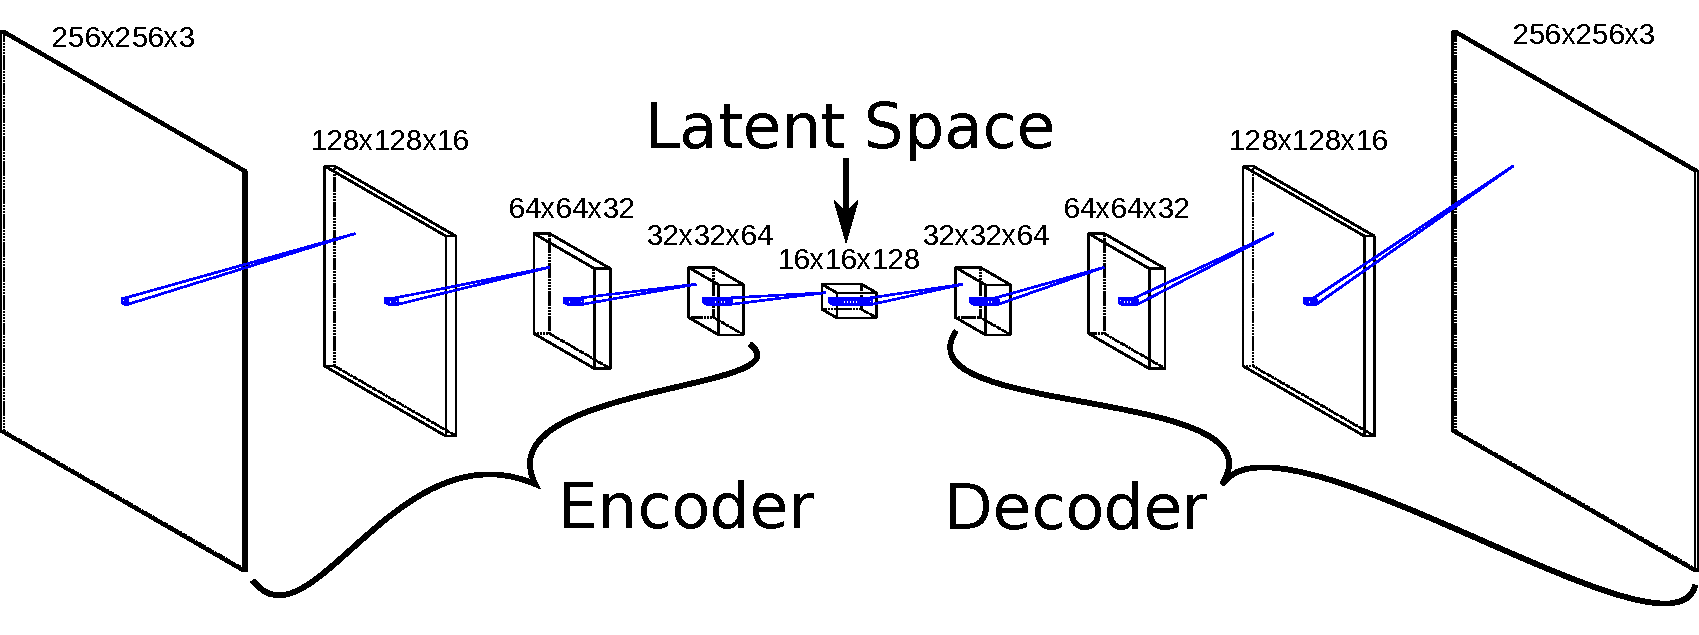
\includegraphics[width=1\linewidth]{figures/models/AutoEncoder.pdf}
    \caption[AutoEncoder]{AutoEncoder architecture\footnotemark{} for images.}
    \label{fig:autoencoder_schema}
\end{figure}

\footnotetext{\href{https://awesomeopensource.com/project/yu4u/convnet-drawer?categoryPage=11}{https://awesomeopensource.com/project/yu4u/convnet-drawer?categoryPage=11}}
